% Shared standalone design for the editable figure reconstructions.
\documentclass[tikz,border=5pt,10pt]{standalone}
\usepackage[T1]{fontenc}
\usepackage[utf8]{inputenc}
\usepackage{newpxtext,newpxmath}
\usepackage[scaled=.94]{sourcesanspro}
\usepackage{pgfplots}
\pgfplotsset{compat=1.18}
\usetikzlibrary{arrows.meta,calc,positioning,decorations.pathreplacing,
  decorations.markings,patterns,matrix,shapes.geometric,fit,backgrounds,
  intersections,angles,quotes}
\definecolor{ink}{HTML}{203746}
\definecolor{accent}{HTML}{146C78}
\definecolor{muted}{HTML}{667780}
\definecolor{signalred}{HTML}{B94B44}
\color{ink}
\tikzset{>=Latex,line width=.8pt,
  every node/.style={font=\small},
  axis/.style={->,draw=muted,line width=.5pt},
  guide/.style={draw=muted,dashed,line width=.45pt},
  curve/.style={draw=accent,line width=1pt},
  marker/.style={circle,fill=accent,inner sep=1.5pt},
  labelbox/.style={fill=white,inner sep=2pt}}

\begin{document}
\begin{tikzpicture}
\path[use as bounding box] (-.6,-.65) rectangle (10.5,5.4);
\path[fill=accent!5,draw=muted!55,dashed,line width=.4pt]
  (1.4,4.4)--(6.4,3.4)--(4.4,2.4)--cycle;
\coordinate (X) at (3.4,.4);\fill[ink] (X) circle (2pt) node[below] {$x$};
\draw[->,accent,line width=1pt] (X)--(1.4,4.4) node[above] {$\nabla f_1(x)$};
\draw[->,accent,line width=1pt] (X)--(6.4,3.4) node[above] {$\nabla f_2(x)$};
\draw[->,accent,line width=1pt] (X)--(4.4,2.4) ;\node[anchor=west] at (4.5,2.85) {$\nabla f_3(x)$};
\draw[->,signalred,dashed,line width=1.5pt] (X)--(4.066667,3.4);
\node[signalred] at (3.5,3.6) {$\nabla f(x)$};
\node[anchor=west] at (6.35,1.7) {$f=\tfrac13(f_1+f_2+f_3)$};
\node[anchor=west] at (6.35,1.1) {$i\sim\operatorname{Unif}\{1,2,3\}$};
\node at (4.8,5) {$\mathbb E_i[\nabla f_i(x)]=\nabla f(x)$};
\end{tikzpicture}
\end{document}
